\chapter{Implementación de SMMD}

A continuación de describe la estructura de la implementación del Sistema Modular de métricas de desempeño en el CECAD.
Se describe una arquitectura de tipo cliente/servidor, donde el servidor es el equipo del investigador, y los clientes son los nodos
que le han sido asignados para trabajar dentro del centro de computación de alto desempeño.


\subsection{Requisitos mínimos del sistema}
Para hacer uso de SSMD el sistema operativo deberá tener los siguientes requerimientos minímos para poder ser instalado y utilizado.
Estos requisitos se dividen en requisitos del servidor y cliente.

\subsubsection{Requisitos del Servidor}
Los siguientes son los requisitos de software para instalar el software servidor de SSMD.

\begin{enumerate}
	\item Docker Community Edition. Disponible para su descarga en \url{https://docs.docker.com/install}
	\item Python 2.7. Disponible para su descarga en \url{https://www.python.org/downloads/}
	\item Ansible. Ver \url{https://docs.ansible.com/ansible/latest/installation_guide/intro_installation.html}
	\item Requisitos opcionales 
	\begin{itemize}
		\item Virtualbox \url{https://www.virtualbox.org/wiki/Downloadsre}
		\item Vagrant \url{https://www.vagrantup.com/downloads.html}
	\end{itemize}
\end{enumerate}

\subsubsection{Requisitos del Cliente}
Los siguientes son los requisitos de software para instalar el software servidor de SSMD.
\begin{enumerate}
	\item Python 2.7. Disponible para su descarga en \url{https://www.python.org/downloads/}
	\item Acceso SSH habilitado para conexiones salientes.
    \item Sistema Operativo CentOS 7 o Ubuntu 16.04 LTS (Xenial Xersus) 
    \begin{itemize}
    	\item CentosOS: \url{https://www.centos.org/download/}
    	\item Ubuntu: \url{http://releases.ubuntu.com/16.04/}
    \end{itemize}
\end{enumerate}


\section{Fuentes de Instalación}\label{fuentes-instalacion}
El código fuente de este proyecto se encuentra en el repositorio público \url{https://github.com/bizoru/ssmd}, este puede ser descargado desde cualquier lugar 
y está disponible con uso de licencia GNU GPL v3.\footnote{Licencia Pública General GNU https://www.gnu.org/licenses/gpl-3.0.en.html}
\\\\
La estructura del código se puede visualizar en la Figura \ref{fig:estructura-fuente}

\begin{figure}[h]
 \centering
  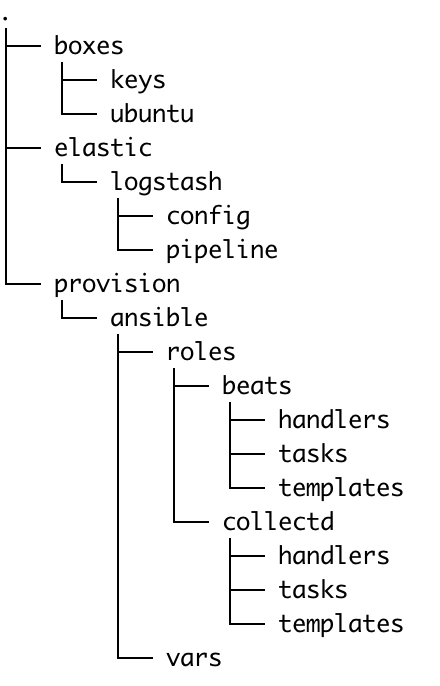
\includegraphics[width=0.3\linewidth]{./imagenes/estructura-fuente.png}
  \caption{Instalación de SMMD en Nodos Cliente.}
  \label{fig:estructura-fuente}
\end{figure}

A continuación se describe la estructura de archivos que se encuentran en el código fuente de acuerdo con su funcionalidad y propósito.

\newpage

Las carpetas que se encuentran en el código fuente de acuerdo con la figura \ref{fig:estructura-fuente} son:

\begin{itemize}
	\item boxes
    \begin{itemize}
      \item[] Esta carpeta contiene las imágenes de \gls{vagrant} para hacer la demostración de SMMD sin necesidad de tener nodos externos. Contiene las llaves SSH \footnote{SSH, Secure Shell, Protocolo para operar computadoras a través de la red de manera segura.} que se utilizarán para acceder a los nodos y la definición de los mismos.
    \end{itemize}
    \item elastic
    \begin{itemize}
      \item[] Esta carpeta contiene el archivo principal de \gls{docker_compose} el cual contiene las imágenes de Logstash, Kibana, y Elastic Search, aquí se encuentra toda la configuración de puertos, nombre del cluster y contraseña de acceso para el sistema de SMMD a través de Kibana.
    \end{itemize}
    \item provision
    \begin{itemize}
      \item[] Esta carpeta contiene los scripts\footnote{Conjunto de \gls{script}s que permite la automatización de procesos.} de aprovisionamiento, allí se encuentran dividos en unidades lógicas llamados roles, estos definen que componente del cliente se va a instalar, para este caso, el demonio Collectd (Ver sección \ref{demonio-collectd}) y MetricBeat (Ver sección \ref{metricbeat}). También encontramos la definición de las variables de cada uno de los programas a instalar, y las configuraciones especificas tanto para Collectd como para metricbeat.
    \end{itemize}
\end{itemize}

\section{Instalación}
La instalación de SMMD consta de dos etapas: La primera etapa consiste en la descarga de la fuente de instalación, (Ver sección \ref{fuentes-instalacion}) preparar los requisitos
de instalación del servidor de acuerdo al sistema operativo del investigador, posteriormente se deben subir los servicios de Logstash (Ver sección \ref{logstash-description}), Elastic Search (Ver sección \ref{elastic-search} ) y Kibana (Ver sección \ref{kibana}).

\subsection{Instalación del Servidor SMMD}
Es importante tener en cuenta los siguientes puntos en consideración para que el proceso de instalación del servidor se pueda realizar a cabo sin problema:
\begin{enumerate}
	\item Habilitar las reglas de firewall para que pueda tener comunicación con los diferentes nodos.
\end{enumerate}
Para proceder con la iniciación de los servicios de Kibana, ElasticSearch y Logstash realice los siguientes pasos:

\begin{enumerate}
	\item Ingrese a la carpeta \texttt{elastic}
	\item Ejecute el comando \texttt{docker-compose up}
\end{enumerate}

\begin{figure}[h]
 \centering
  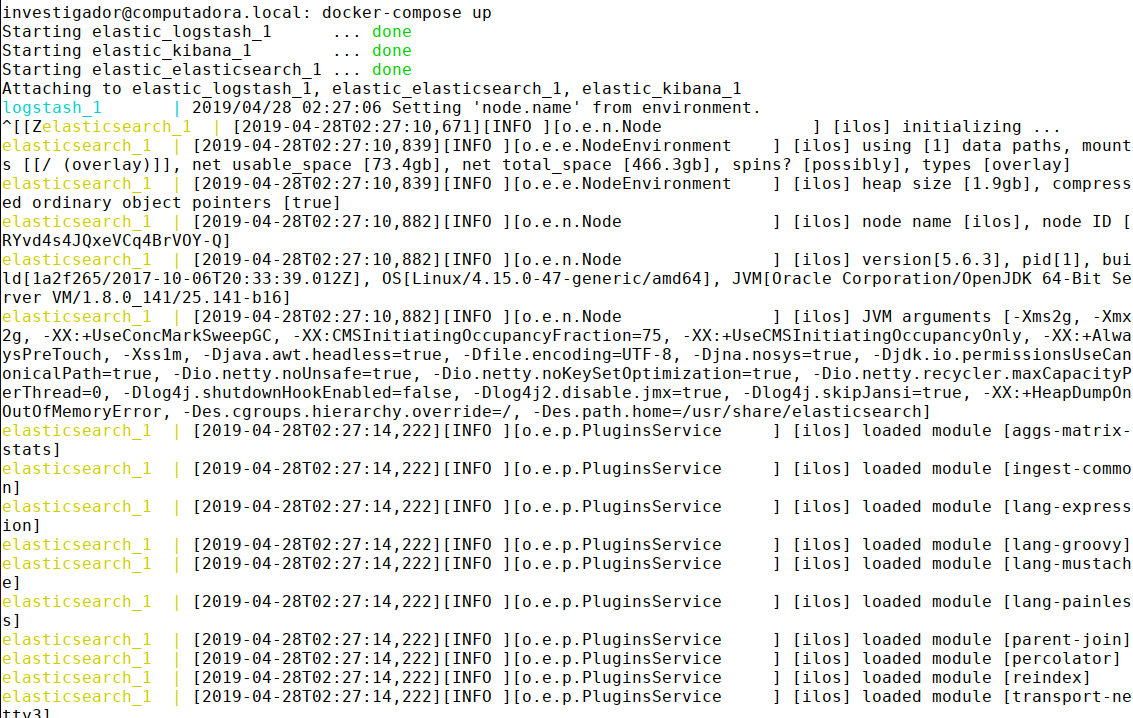
\includegraphics[width=0.85\linewidth]{./imagenes/docker-compose-up.png}
  \caption{Ejemplo, resultado de la ejecución de docker-compose up, iniciación de servicios}
  \label{fig:docker-compose-up}
\end{figure}

El proceso tomará algun tiempo en completarse una vez esta haya finalizado podrá acceder la interfaz de administración ingresando a \url{http://localhost:5601}, el usuario es \textit{elastic} y la contraseña es \textit{changeme}.

\begin{figure}[h]
 \centering
  
\includegraphics[width=0.4\linewidth]{./imagenes/login-page.png}
  \caption{Pantalla de inicio de sesión en Kibana}
  \label{fig:kibana-login-page}
\end{figure}

Con estos pasos se ha completado la instalación del servidor central donde el investigador podrá acceder al panel de administración y visualizar las métricas de desempeño.

\newpage
\subsection{Aprovisionamiento de Nodos}
SMMD provee una herramienta para hacer la instalación de Metricbeat y collectd, a través de un script de aprovisionamiento dicho script establecerá una conexión SSH hacia los nodos en el cluster y utilizando Ansible hará la instalación del software requerido y configurará los valores necesarios para la comunicación con el servidor central.

\begin{figure}[ht]
 \centering
  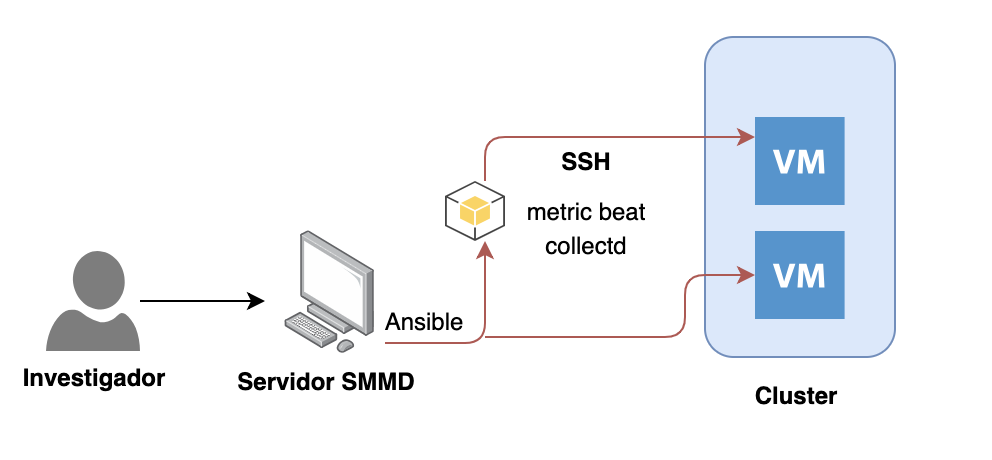
\includegraphics[width=0.5\linewidth]{./imagenes/modelo-instalacion.png}
  \caption{Instalación de SMMD en Nodos Cliente.}
  \label{fig:modelo-instalacion}
\end{figure}

Las siguientes son consideraciones importantes ha tener en cuenta para aprovisionar los nodos que enviarán las métricas de desempeño al nodo central.
\begin{enumerate}
	\item El servidor SMMD deberá estar en la misma red en la que están los nodos, con el fin de poder recibir las métricas de desempeño a través de la red.
	\item Cada nodo deberá tener una llave de acceso \gls{ssh} en el archivo \texttt{./ssh/authorized\_keys} con un usuario con permisos de administración.
	\item Habilitar el usuario super administrador y llaves SSH
	\item Habilitar reglas de firewall para habilitar comunicación externa con el servidor central.
	\item Configuración especial en métricas de collectd que se requieran para utilizar en Elastic Search.
\end{enumerate}

Como se puede ver en la figura \ref{fig:modelo-instalacion} el investigador ejecuta el código de aprovisionamiento de \gls{ansible} y este se encarga de hacer la instalación de los paquetes collectd y metricbeat en los nodos o máquinas virtuales que le han sido asignadas en el cluster HPC.

\newpage

El proceso de aprovisionamiento utiliza el script que se encuentra en la ruta \texttt{/provision/provision.sh}, este script se ejecuta de la siguiente manera:

\begin{verbatim}
     export ELASTIC_SEARCH_SERVER=<ip>
     export LOGSTASH_SERVER=<ip>
     provision.sh <host>
\end{verbatim}

Donde las variables para \texttt{ELASTIC\_SEARCH\_SERVER} y \texttt{LOGSTASH\_SERVER} en el campo de \texttt{ip} debe asignarse el valor de la ip pública del servidor en el cual se está ejecutando el script de aprovisionamiento.

\begin{figure}[h]
 \centering
  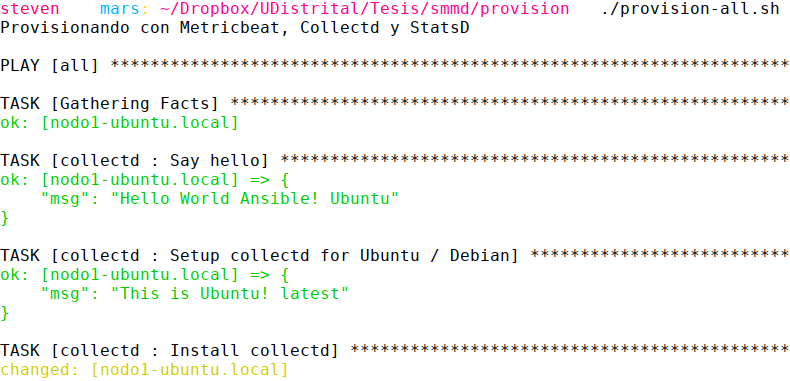
\includegraphics[width=0.6\linewidth]{./imagenes/provision_all.png}
  \caption{Aprovisionamiento de SMMD en los nodos cliente.}
  \label{fig:aprovisionamiento-nodos}
\end{figure}
Como se puede ver en la figura \ref{fig:aprovisionamiento-nodos} este es el resultado que entrega la consola en el momento de ejecutar el aprovisionamiento, al final del proceso, todos los nodos que hayan sido provisionados, tendrán activos los servicios de metricbeat, collectd y statsd.
\clearpage

\section{Uso}
A continuación se describe el uso de SMMD
\subsection{Visualización de Métricas de Desempeño}
asdf
Seleccionar las métricas de desempeño de cada nodo según el nombre de host asignado.
\begin{figure}[h]
 \centering
  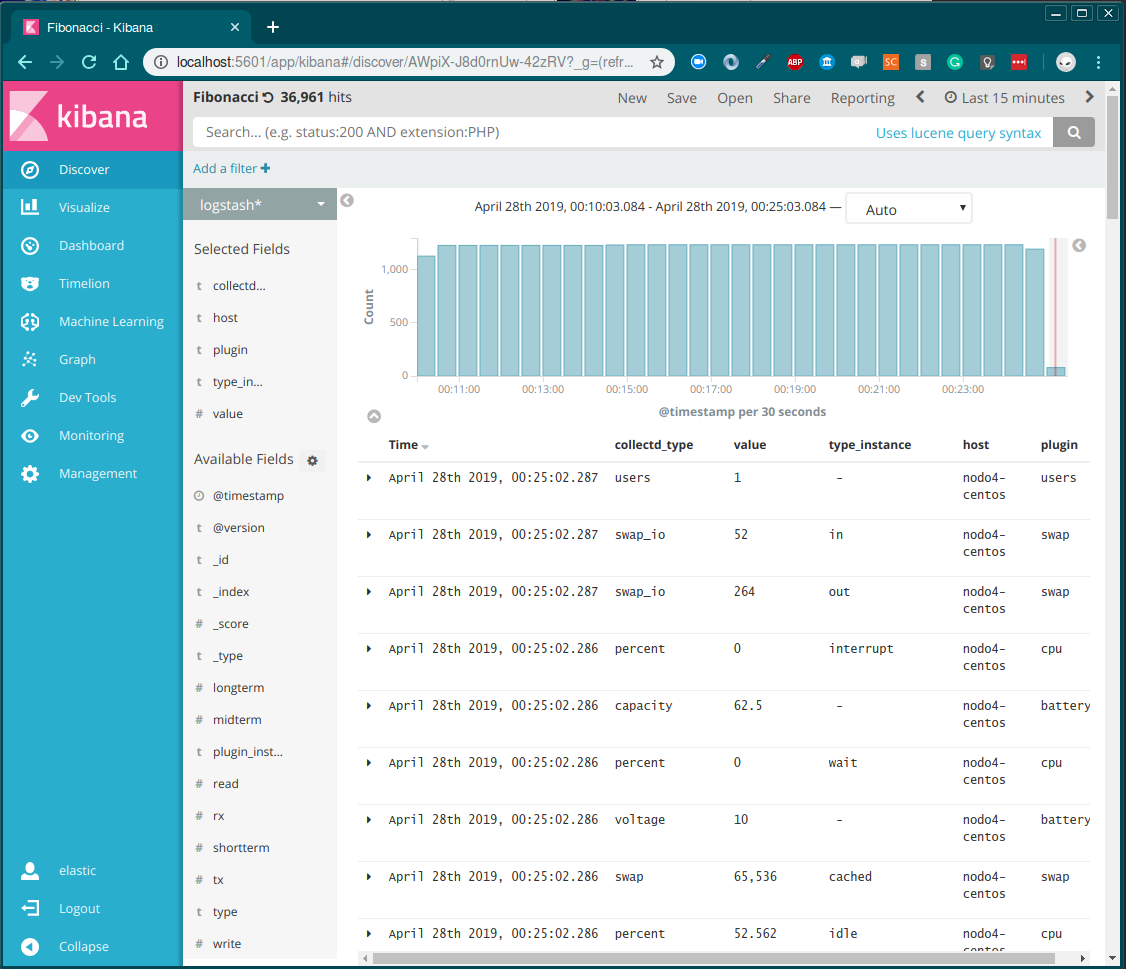
\includegraphics[width=0.6\linewidth]{./imagenes/kibana-home.png}
  \caption{Pantalla Principal de SMMD}
  \label{fig:home-smmd}
\end{figure}

\newpage

\subsection{Ajustes generales}
Ajustes generales a nivel del motor de base de datos no relacional Elastic Seach para el almacenamiento de la información de las métricas de desempeño.


\subsection{Plugins}

Ajustes generales a nivel de plugin del lado del cliente. Inclusión de nuevas métricas y valores especificos en la configuración del demonio collectd.




